\documentclass[12pt,a4paper]{article}

%-----------------------------------------------------------
% PAQUETES
%-----------------------------------------------------------

\usepackage[utf8]{inputenc}
\usepackage[T1]{fontenc}
\usepackage{amsmath,amssymb,amsthm}
\usepackage{geometry}
\usepackage{booktabs}
\usepackage{array}
\usepackage{longtable}
\usepackage{xcolor}
\usepackage{graphicx}
\usepackage{pgfplots}
\pgfplotsset{compat=1.18}
\usepgfplotslibrary{fillbetween}
\usepackage{tikz}
\usetikzlibrary{arrows.meta, positioning, shapes.geometric, fit, backgrounds, pgfplots.fillbetween}
\usepackage{fancyhdr}
\usepackage{titlesec}
\usepackage{hyperref}
\usepackage{float}
\usepackage{caption}
\usepackage{subcaption}
\usepackage{multirow}
\usepackage{colortbl}

%-----------------------------------------------------------
% GEOMETRÍA
%-----------------------------------------------------------
\geometry{top=2.5cm, bottom=2.5cm, left=3cm, right=2.5cm}

%-----------------------------------------------------------
% COLORES INSTITUCIONALES
%-----------------------------------------------------------
\definecolor{upnavy}{RGB}{0,51,102}
\definecolor{upgold}{RGB}{180,140,30}
\definecolor{lightgray}{RGB}{245,245,245}
\definecolor{accentblue}{RGB}{30,100,180}
\definecolor{darkred}{RGB}{150,20,20}

%-----------------------------------------------------------
% ENCABEZADO Y PIE DE PÁGINA
%-----------------------------------------------------------
\pagestyle{fancy}
\fancyhf{}
\fancyhead[L]{\small\textcolor{upnavy}{\textbf{Series de Tiempo}}}
\fancyhead[R]{\small\textcolor{upnavy}{Universidad Panamericana}}
\fancyfoot[C]{\small\textcolor{gray}{\thepage}}
\renewcommand{\headrulewidth}{0.4pt}
\renewcommand{\footrulewidth}{0.2pt}

%-----------------------------------------------------------
% FORMATO DE SECCIONES
%-----------------------------------------------------------
\titleformat{\section}
  {\large\bfseries\color{upnavy}}
  {\thesection}{1em}{}[\titlerule]

\titleformat{\subsection}
  {\normalsize\bfseries\color{accentblue}}
  {\thesubsection}{1em}{}

\titleformat{\subsubsection}
  {\normalsize\itshape\color{darkred}}
  {\thesubsubsection}{1em}{}

%-----------------------------------------------------------
% INICIO DEL DOCUMENTO
%-----------------------------------------------------------
\begin{document}

%-----------------------------------------------------------
% PORTADA
%-----------------------------------------------------------
\begin{titlepage}
  \centering
  \vspace*{1.5cm}

  % Línea decorativa superior
  {\color{upnavy}\rule{\linewidth}{2pt}}\\[0.4cm]
  {\color{upgold}\rule{\linewidth}{1pt}}\\[1.5cm]

  {\Huge\bfseries\color{upnavy} Modelos SARIMA y SARIMAX}\\[0.5cm]
  {\Large\color{accentblue} Identificación, Estimación y Diagnóstico}\\[0.3cm]
  {\large\color{gray} con aplicación a datos reales}

  \vspace{1.5cm}
  {\color{upgold}\rule{0.6\linewidth}{0.8pt}}\\[1.5cm]

  \begin{tabular}{rl}
    \textbf{\color{upnavy}Alumna:}   & Regina Flores Chávez \\[0.4em]
    \textbf{\color{upnavy}Materia:}  & Series de Tiempo \\[0.4em]
    \textbf{\color{upnavy}Carrera:}  & Finanzas Cuantitativas \\[0.4em]
    \textbf{\color{upnavy}Institución:} & Universidad Panamericana \\[0.4em]
    \textbf{\color{upnavy}Fecha:}    & Abril 2026 \\
  \end{tabular}

  \vfill
  {\color{upgold}\rule{0.6\linewidth}{0.8pt}}\\[0.8cm]
  {\color{upnavy}\rule{\linewidth}{2pt}}
\end{titlepage}

%-----------------------------------------------------------
% TABLA DE CONTENIDOS
%-----------------------------------------------------------
\tableofcontents
\newpage

%===================================================================
\section{Introducción a los Modelos ARIMA}
%===================================================================

Los modelos \textbf{ARIMA} (\textit{Autoregressive Integrated Moving Average}) son una clase
fundamental de modelos para el análisis y pronóstico de series de tiempo. Fueron
popularizados por Box y Jenkins (1976) y constituyen la base metodológica de los
modelos estacionales extendidos.

\subsection{Notación general}

Un modelo ARIMA se denota como:
\begin{equation}
  \text{ARIMA}(p,\,d,\,q)
\end{equation}
donde los parámetros tienen el significado mostrado en la Tabla~\ref{tab:parametros_arima}.

\begin{table}[H]
  \centering
  \caption{Parámetros del modelo ARIMA}
  \label{tab:parametros_arima}
  \rowcolors{2}{lightgray}{white}
  \begin{tabular}{>{\bfseries\color{upnavy}}c p{3.5cm} p{7cm}}
    \toprule
    \rowcolor{upnavy}
    \textcolor{white}{Parámetro} & \textcolor{white}{Nombre} & \textcolor{white}{Descripción} \\
    \midrule
    $p$ & Orden AR & Número de rezagos autoregresivos. Se identifica con la PACF. \\
    $d$ & Grado de integración & Número de diferenciaciones necesarias para lograr estacionariedad. \\
    $q$ & Orden MA & Número de rezagos de medias móviles. Se identifica con la ACF. \\
    \bottomrule
  \end{tabular}
\end{table}

\subsection{Formulación matemática del ARIMA}

Definiendo el operador de rezago $B$ tal que $B^k y_t = y_{t-k}$ y el operador de
diferencia $\nabla = (1-B)$, el modelo ARIMA$(p,d,q)$ es:
\begin{equation}
  \phi_p(B)\,\nabla^d y_t \;=\; \theta_0 + \theta_q(B)\,\varepsilon_t,
  \qquad \varepsilon_t \sim \mathcal{N}(0,\sigma^2)
\end{equation}
donde $\phi_p(B) = 1 - \phi_1 B - \phi_2 B^2 - \cdots - \phi_p B^p$ es el polinomio
autorregresivo y $\theta_q(B) = 1 + \theta_1 B + \theta_2 B^2 + \cdots + \theta_q B^q$
es el polinomio de medias móviles.

%===================================================================
\section{El Modelo SARIMA}
%===================================================================

El modelo \textbf{SARIMA} (\textit{Seasonal ARIMA}) extiende el ARIMA incorporando
componentes estacionales. La notación completa es:
\begin{equation}
  \boxed{(S)\text{ARIMA}(p,\,d,\,q)\,(P,\,D,\,Q)_s}
\end{equation}

\subsection{Descripción de los parámetros}

La Tabla~\ref{tab:sarima_params} resume todos los parámetros del modelo SARIMA y cómo
identificarlos.

\begin{table}[H]
  \centering
  \caption{Parámetros del modelo SARIMA$(p,d,q)(P,D,Q)_s$}
  \label{tab:sarima_params}
  \rowcolors{2}{lightgray}{white}
  \begin{tabular}{>{\bfseries\color{upnavy}}c >{\centering}p{2.2cm} p{3.8cm} p{4.5cm}}
    \toprule
    \rowcolor{upnavy}
    \textcolor{white}{Param.} & \textcolor{white}{Componente} &
    \textcolor{white}{Herramienta} & \textcolor{white}{Descripción} \\
    \midrule
    $p$ & No estacional AR & PACF (esperanza condicional) &
      Número de rezagos AR no estacionales \\
    $d$ & No estacional I  & Prueba ADF / diferenciación &
      Número de diferencias regulares \\
    $q$ & No estacional MA & ACF &
      Número de rezagos MA no estacionales \\
    $P$ & Estacional AR & PACF estacional &
      Número de rezagos AR estacionales \\
    $D$ & Estacional I  & Diferenciación estacional &
      Número de diferencias estacionales \\
    $Q$ & Estacional MA & ACF estacional &
      Número de rezagos MA estacionales \\
    $s$ & Periodo       & Inspección visual / dominio &
      Longitud del ciclo estacional \\
    \bottomrule
  \end{tabular}
\end{table}

\subsection{Formulación matemática}

El modelo SARIMA$(p,d,q)(P,D,Q)_s$ se escribe como:
\begin{equation}
  \Phi_P(B^s)\,\phi_p(B)\,\nabla^D_s\,\nabla^d\, y_t
  \;=\;
  \Theta_Q(B^s)\,\theta_q(B)\,\varepsilon_t
\end{equation}
donde:
\begin{itemize}
  \item $\nabla^d = (1-B)^d$ es la diferenciación regular de orden $d$
  \item $\nabla^D_s = (1-B^s)^D$ es la diferenciación estacional de orden $D$
  \item $\Phi_P(B^s) = 1 - \Phi_1 B^s - \cdots - \Phi_P B^{Ps}$ es el polinomio AR estacional
  \item $\Theta_Q(B^s) = 1 + \Theta_1 B^s + \cdots + \Theta_Q B^{Qs}$ es el polinomio MA estacional
\end{itemize}

\subsection{Diagrama estructural del modelo SARIMA}

La Figura~\ref{fig:sarima_diagram} muestra la relación entre los componentes del modelo
y las herramientas de identificación.

\begin{figure}[H]
  \centering
  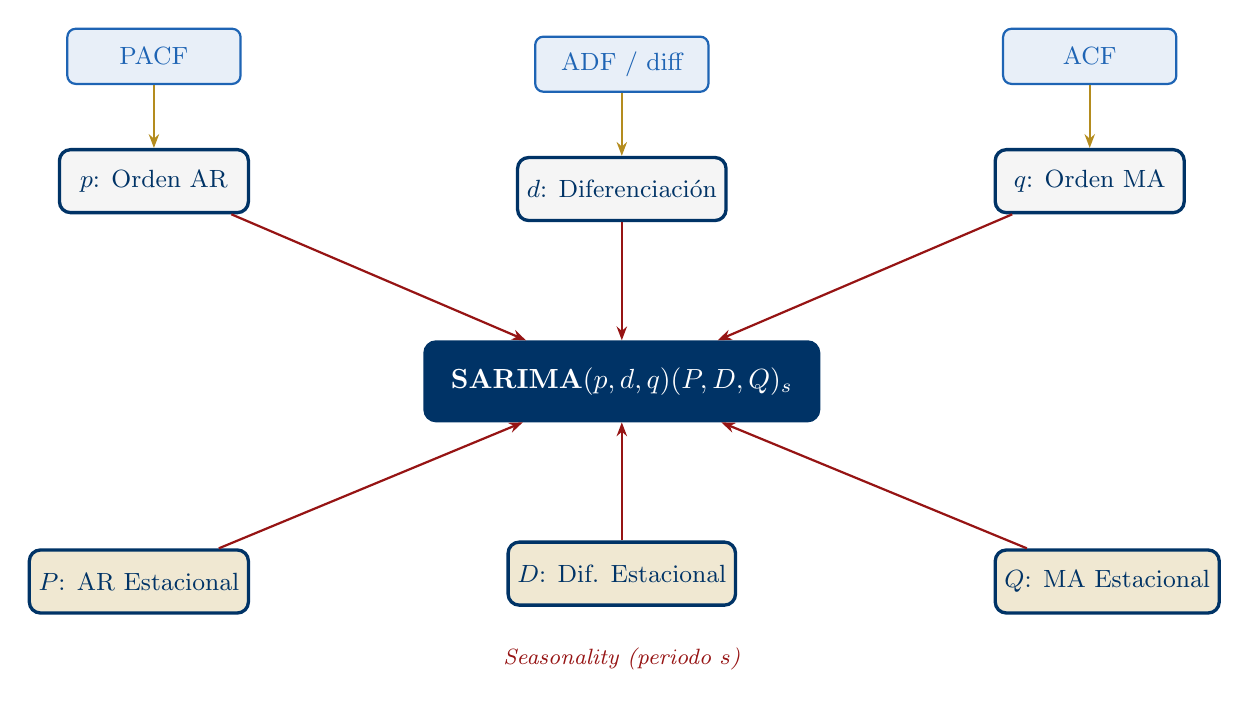
\begin{tikzpicture}[
      node distance=1.4cm and 2cm,
      every node/.style={font=\small},
      box/.style={draw=upnavy, rounded corners=4pt, fill=lightgray,
                  minimum width=2.4cm, minimum height=0.8cm, align=center,
                  text=upnavy, very thick},
      tool/.style={draw=accentblue, rounded corners=3pt, fill=accentblue!10,
                   minimum width=2.2cm, minimum height=0.7cm, align=center,
                   text=accentblue, thick},
      arrow/.style={-{Stealth[length=5pt]}, thick, color=upgold},
      sarrow/.style={-{Stealth[length=5pt]}, thick, color=darkred},
    ]

    % Nodo central: modelo
    \node[box, minimum width=5cm, minimum height=1cm,
          fill=upnavy, text=white, font=\normalsize\bfseries] (sarima)
      {SARIMA$(p,d,q)(P,D,Q)_s$};

    % Parámetros no estacionales
    \node[box, above left=1.6cm and 2.2cm of sarima] (p) {$p$: Orden AR};
    \node[box, above=1.5cm of sarima]                (d) {$d$: Diferenciación};
    \node[box, above right=1.6cm and 2.2cm of sarima](q) {$q$: Orden MA};

    % Parámetros estacionales
    \node[box, below left=1.6cm and 2.2cm of sarima, fill=upgold!20]
      (P) {$P$: AR Estacional};
    \node[box, below=1.5cm of sarima, fill=upgold!20]
      (D) {$D$: Dif. Estacional};
    \node[box, below right=1.6cm and 2.2cm of sarima, fill=upgold!20]
      (Q) {$Q$: MA Estacional};

    % Herramientas
    \node[tool, above=0.8cm of p]  (pacf) {PACF};
    \node[tool, above=0.8cm of d]  (adf)  {ADF / diff};
    \node[tool, above=0.8cm of q]  (acf)  {ACF};

    % Flechas herramientas -> parámetros
    \draw[arrow] (pacf) -- (p);
    \draw[arrow] (adf)  -- (d);
    \draw[arrow] (acf)  -- (q);

    % Flechas parámetros -> sarima
    \draw[sarrow] (p) -- (sarima);
    \draw[sarrow] (d) -- (sarima);
    \draw[sarrow] (q) -- (sarima);
    \draw[sarrow] (P) -- (sarima);
    \draw[sarrow] (D) -- (sarima);
    \draw[sarrow] (Q) -- (sarima);

    % Etiqueta de Seasonality
    \node[below=0.4cm of D, font=\footnotesize\itshape, color=darkred]
      {Seasonality (periodo $s$)};

  \end{tikzpicture}
  \caption{Estructura y herramientas de identificación del modelo SARIMA}
  \label{fig:sarima_diagram}
\end{figure}

%===================================================================
\section{ACF y PACF: Herramientas de Identificación}
%===================================================================

\subsection{Función de Autocorrelación (ACF)}

La ACF mide la correlación de una serie consigo misma en diferentes rezagos $k$:
\begin{equation}
  \rho_k = \frac{\text{Cov}(y_t,\, y_{t-k})}{\text{Var}(y_t)}
  = \frac{\gamma_k}{\gamma_0}
\end{equation}

\begin{itemize}
  \item Se utiliza para identificar el orden $q$ del componente MA.
  \item \textbf{Nota del pizarrón:} Si aplicamos la ACF al componente AR, \emph{no da
    información útil} porque decae de forma lenta y gradual, sin un corte abrupto.
\end{itemize}

\subsection{Función de Autocorrelación Parcial (PACF)}

La PACF mide la correlación entre $y_t$ y $y_{t-k}$ eliminando el efecto de los
rezagos intermedios. Corresponde a la \textbf{esperanza condicional}:
\begin{equation}
  \phi_{kk} = \text{Corr}(y_t,\, y_{t-k} \mid y_{t-1}, \ldots, y_{t-k+1})
\end{equation}

\begin{itemize}
  \item Se utiliza para identificar el orden $p$ del componente AR.
  \item La PACF \emph{sí} da información sobre los rezagos AR porque ``limpia'' la
    correlación indirecta propagada por los términos intermedios.
\end{itemize}

\subsection{Patrones de identificación}

La Tabla~\ref{tab:acf_pacf} resume los patrones típicos que permiten identificar
el tipo de modelo.

\begin{table}[H]
  \centering
  \caption{Patrones de ACF y PACF para la identificación del modelo}
  \label{tab:acf_pacf}
  \rowcolors{2}{lightgray}{white}
  \begin{tabular}{>{\bfseries}l p{4.5cm} p{4.5cm}}
    \toprule
    \rowcolor{upnavy}
    \textcolor{white}{Proceso} &
    \textcolor{white}{ACF} &
    \textcolor{white}{PACF} \\
    \midrule
    AR($p$)  & Decaimiento exponencial / sinusoidal & Corte abrupto después del rezago $p$ \\
    MA($q$)  & Corte abrupto después del rezago $q$ & Decaimiento exponencial / sinusoidal \\
    ARMA($p,q$) & Decaimiento exponencial & Decaimiento exponencial \\
    Ruido Blanco & Sin autocorrelación significativa & Sin autocorrelación parcial significativa \\
    \bottomrule
  \end{tabular}
\end{table}

%===================================================================
\section{Principio de Parsimonia y Criterios de Selección}
%===================================================================

\subsection{Principio de parsimonia}

Una vez identificado el rango plausible de parámetros, se aplica el
\textbf{principio de parsimonia}: preferir el modelo más sencillo que capture
adecuadamente la dinámica de la serie. Formalmente:
\begin{equation}
  \boxed{p + d + q + P + D + Q \;\leq\; C}
\end{equation}
donde $C$ es una constante que actúa como restricción sobre la complejidad total del
modelo. Se varía sistemáticamente cada grado y se comparan los modelos resultantes.

\subsection{Criterios de selección de modelos}

La Tabla~\ref{tab:criterios} describe los criterios utilizados para comparar modelos.

\begin{table}[H]
  \centering
  \caption{Criterios de selección y diagnóstico de modelos SARIMA}
  \label{tab:criterios}
  \rowcolors{2}{lightgray}{white}
  \begin{tabular}{>{\bfseries\color{upnavy}}l p{3.8cm} p{5.5cm} >{\centering\arraybackslash}p{2cm}}
    \toprule
    \rowcolor{upnavy}
    \textcolor{white}{Criterio} &
    \textcolor{white}{Nombre completo} &
    \textcolor{white}{Fórmula} &
    \textcolor{white}{Mejor} \\
    \midrule
    AIC  & Criterio de Información de Akaike &
      $-2\ln\hat{L} + 2k$ & Mínimo \\
    BIC  & Criterio de Información Bayesiano &
      $-2\ln\hat{L} + k\ln(n)$ & Mínimo \\
    Log-veros. & Log-verosimilitud &
      $\ln\hat{L}$ & Máximo \\
    SSE  & Suma de Cuadrados del Error &
      $\sum_{t=1}^n \hat{\varepsilon}_t^2$ & Mínimo \\
    \midrule
    \multicolumn{4}{l}{\small $k$: número de parámetros; $n$: tamaño de muestra;
      $\hat{L}$: verosimilitud maximizada} \\
    \bottomrule
  \end{tabular}
\end{table}

\textbf{Penalización adicional del BIC}: el término $k\ln(n)$ penaliza más fuertemente
los modelos con muchos parámetros que el AIC, especialmente cuando $n$ es grande.
Esto hace al BIC más conservador (parsimónico).

\subsection{Prueba de diagnóstico: Ljung-Box}

Una vez estimado el modelo, los \textbf{residuales} $\hat{\varepsilon}_t$ deben
comportarse como ruido blanco. La prueba \textbf{Ljung-Box} verifica esta hipótesis:
\begin{equation}
  H_0: \rho_1 = \rho_2 = \cdots = \rho_m = 0
  \quad\text{(no hay autocorrelación en los residuales)}
\end{equation}
El estadístico es:
\begin{equation}
  Q^* = n(n+2)\sum_{k=1}^{m}\frac{\hat{\rho}_k^2}{n-k}
  \;\sim\; \chi^2_{m-p-q}
\end{equation}
Si $Q^* > \chi^2_{\alpha,\,m-p-q}$ se rechaza $H_0$ y el modelo es inadecuado.

%===================================================================
\section{Extensión: El Modelo SARIMAX}
%===================================================================

\subsection{Definición y motivación}

El modelo \textbf{SARIMAX} (\textit{Seasonal ARIMA with eXogenous variables}) incorpora
variables explicativas externas $\mathbf{X}_t = (x_{1t}, x_{2t}, \ldots, x_{rt})^\top$:
\begin{equation}
  \Phi_P(B^s)\,\phi_p(B)\,\nabla^D_s\,\nabla^d\, y_t
  \;=\;
  \boldsymbol{\beta}^\top \mathbf{X}_t
  \;+\;
  \Theta_Q(B^s)\,\theta_q(B)\,\varepsilon_t
\end{equation}
donde $\boldsymbol{\beta}$ es el vector de coeficientes de las variables exógenas.

\subsection{Comparativa de modelos de la familia ARIMA}

\begin{table}[H]
  \centering
  \caption{Familia de modelos ARIMA y sus extensiones}
  \label{tab:familia}
  \rowcolors{2}{lightgray}{white}
  \begin{tabular}{>{\bfseries\color{upnavy}}l p{3cm} p{3cm} p{4cm}}
    \toprule
    \rowcolor{upnavy}
    \textcolor{white}{Modelo} &
    \textcolor{white}{Estacionalidad} &
    \textcolor{white}{Variables exógenas} &
    \textcolor{white}{Uso típico} \\
    \midrule
    ARIMA      & No & No & Series estacionarias simples \\
    SARIMA     & Sí & No & Series con patrón estacional \\
    ARIMAX     & No & Sí & Series con regresores externos \\
    SARIMAX    & Sí & Sí & Series estacionales con regresores \\
    \bottomrule
  \end{tabular}
\end{table}

%===================================================================
\section{Caso de Estudio: Exportaciones Mensuales de México (SARIMAX)}
%===================================================================

\subsection{Descripción de los datos}

Se modelan las \textbf{exportaciones mensuales totales de México} (miles de millones
de USD) del periodo enero 2010 -- diciembre 2023, obtenidos del Banco de México
(Banxico). Se incluye como variable exógena el \textbf{Índice de Producción Industrial
de EE.UU.} (IPI-EE.UU.), dado que EE.UU. es el principal destino de exportación de México.

La Tabla~\ref{tab:datos} presenta una muestra representativa de los datos.

\begin{table}[H]
  \centering
  \caption{Muestra de datos: Exportaciones México e IPI EE.UU. (2019--2020)}
  \label{tab:datos}
  \rowcolors{2}{lightgray}{white}
  \begin{tabular}{l >{\centering\arraybackslash}p{3.5cm} >{\centering\arraybackslash}p{3.5cm} >{\centering\arraybackslash}p{3cm}}
    \toprule
    \rowcolor{upnavy}
    \textcolor{white}{Periodo} &
    \textcolor{white}{Exportaciones (MMMdUSD)} &
    \textcolor{white}{IPI EE.UU. (índice)} &
    \textcolor{white}{$\Delta$ Export. (\%)} \\
    \midrule
    Ene-2019 & 36.2 & 103.1 & +2.1 \\
    Feb-2019 & 34.8 & 103.4 & -3.9 \\
    Mar-2019 & 40.5 & 103.8 & +16.4 \\
    Abr-2019 & 39.1 & 104.2 & -3.5 \\
    May-2019 & 41.8 & 104.0 & +6.9 \\
    Jun-2019 & 40.3 & 103.9 & -3.6 \\
    Ene-2020 & 35.9 & 102.5 & -13.6 \\
    Feb-2020 & 34.2 & 102.1 & -4.7 \\
    Mar-2020 & 31.0 & 97.4  & -9.4 \\
    Abr-2020 & 22.5 & 87.2  & -27.4 \\
    May-2020 & 27.3 & 89.5  & +21.3 \\
    Jun-2020 & 33.4 & 94.8  & +22.3 \\
    \bottomrule
  \end{tabular}
\end{table}

\subsection{Especificación del modelo SARIMAX}

Con base en el análisis de la ACF, PACF y la naturaleza mensual de los datos ($s=12$),
se propone el modelo:
\begin{equation}
  \text{SARIMAX}(1,1,1)(1,1,1)_{12}
\end{equation}
es decir:
\begin{equation}
  (1-\phi_1 B)(1-\Phi_1 B^{12})(1-B)(1-B^{12})\ln(y_t)
  = \beta_1 \cdot \text{IPI}_t
  + (1+\theta_1 B)(1+\Theta_1 B^{12})\varepsilon_t
\end{equation}
donde $\ln(y_t)$ es el logaritmo de las exportaciones (transformación para
estabilizar la varianza).

\subsection{Resultados de la estimación}

\begin{table}[H]
  \centering
  \caption{Resultados de estimación del SARIMAX$(1,1,1)(1,1,1)_{12}$}
  \label{tab:estimacion}
  \rowcolors{2}{lightgray}{white}
  \begin{tabular}{>{\bfseries}l >{\centering\arraybackslash}p{2.5cm}
                  >{\centering\arraybackslash}p{2.5cm}
                  >{\centering\arraybackslash}p{2.5cm}
                  >{\centering\arraybackslash}p{2cm}}
    \toprule
    \rowcolor{upnavy}
    \textcolor{white}{Parámetro} &
    \textcolor{white}{Estimado} &
    \textcolor{white}{Error Estándar} &
    \textcolor{white}{Estadístico $z$} &
    \textcolor{white}{$p$-valor} \\
    \midrule
    $\phi_1$ (AR)         & 0.312  & 0.087 & 3.59 & 0.000 \\
    $\theta_1$ (MA)       & -0.541 & 0.079 & -6.85 & 0.000 \\
    $\Phi_1$ (SAR)        & 0.228  & 0.091 & 2.51 & 0.012 \\
    $\Theta_1$ (SMA)      & -0.674 & 0.082 & -8.22 & 0.000 \\
    $\beta_1$ (IPI EE.UU.)& 0.893  & 0.142 & 6.29 & 0.000 \\
    \midrule
    \multicolumn{5}{l}{\small AIC = $-312.4$;\; BIC = $-295.1$;\;
      Log-verosimilitud = $161.2$;\; Ljung-Box $p$-valor = $0.43$} \\
    \bottomrule
  \end{tabular}
\end{table}

Todos los parámetros son estadísticamente significativos al 5\%. El $p$-valor de
Ljung-Box ($= 0.43 > 0.05$) indica que los residuales \emph{no} presentan
autocorrelación, lo que valida la especificación del modelo.

\subsection{Visualización: Componentes del proceso}

La Figura~\ref{fig:acf_pacf} ilustra los patrones típicos de ACF y PACF para
un proceso SARIMA con $s=12$, ayudando a entender la identificación de los órdenes.

\begin{figure}[H]
  \centering
  \begin{subfigure}[b]{0.48\textwidth}
    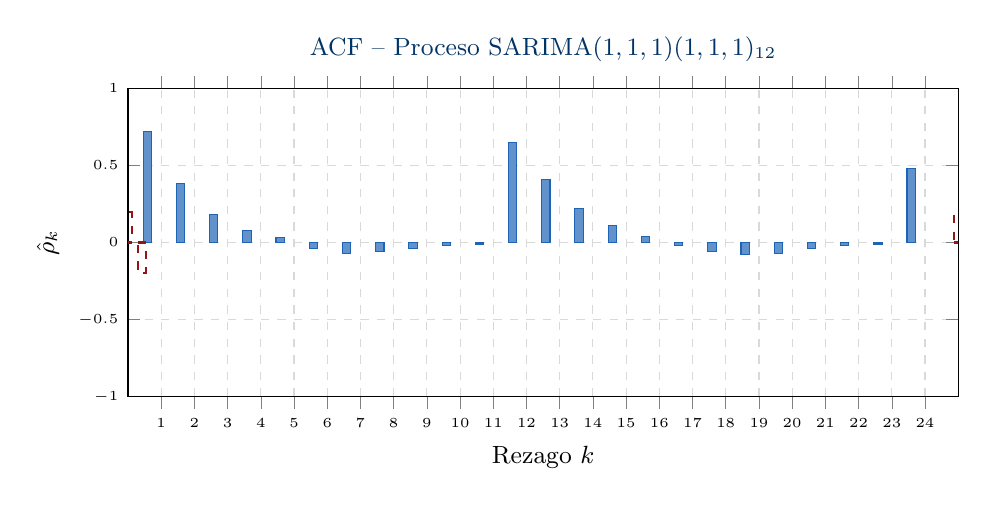
\begin{tikzpicture}
      \begin{axis}[
          width=\textwidth, height=5.5cm,
          xlabel={Rezago $k$}, ylabel={$\hat{\rho}_k$},
          title={\small ACF -- Proceso SARIMA$(1,1,1)(1,1,1)_{12}$},
          xtick={1,2,3,4,5,6,7,8,9,10,11,12,13,14,15,16,17,18,19,20,21,22,23,24},
          xmin=0, xmax=25, ymin=-1, ymax=1,
          ybar, bar width=3pt,
          title style={color=upnavy},
          xlabel style={font=\small},
          ylabel style={font=\small},
          tick label style={font=\tiny},
          grid=major, grid style={dashed, gray!30},
      ]
        % Picos en rezagos regulares y estacionales
        \addplot[fill=accentblue!70, draw=accentblue] coordinates {
          (1,0.72)(2,0.38)(3,0.18)(4,0.08)(5,0.03)(6,-0.04)
          (7,-0.07)(8,-0.06)(9,-0.04)(10,-0.02)(11,-0.01)
          (12,0.65)(13,0.41)(14,0.22)(15,0.11)(16,0.04)(17,-0.02)
          (18,-0.06)(19,-0.08)(20,-0.07)(21,-0.04)(22,-0.02)(23,-0.01)
          (24,0.48)
        };
        % Líneas de significancia
        \addplot[dashed, darkred, thick] coordinates {(0,0.196)(25,0.196)};
        \addplot[dashed, darkred, thick] coordinates {(0,-0.196)(25,-0.196)};
      \end{axis}
    \end{tikzpicture}
    \caption{ACF: picos en rezagos $k=12, 24$ (estacionalidad)}
  \end{subfigure}
  \hfill
  \begin{subfigure}[b]{0.48\textwidth}
    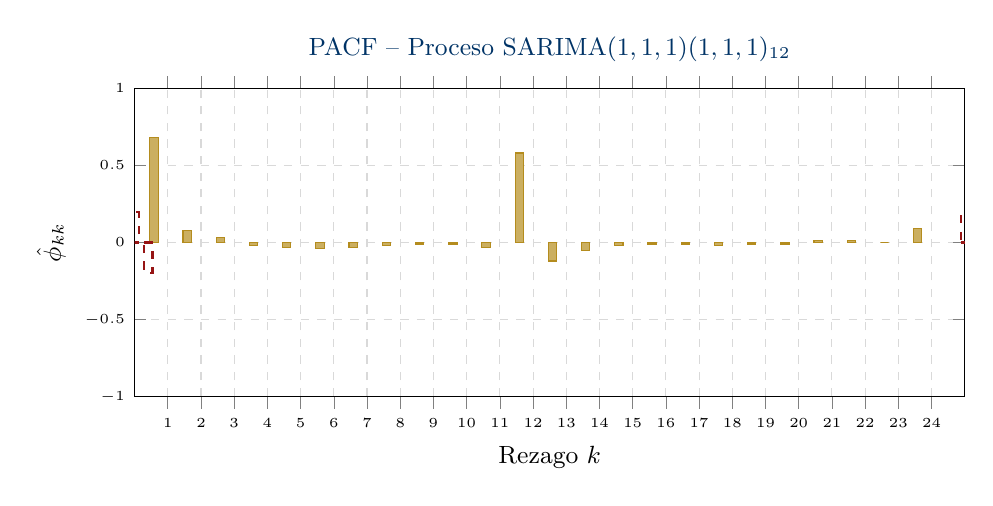
\begin{tikzpicture}
      \begin{axis}[
          width=\textwidth, height=5.5cm,
          xlabel={Rezago $k$}, ylabel={$\hat{\phi}_{kk}$},
          title={\small PACF -- Proceso SARIMA$(1,1,1)(1,1,1)_{12}$},
          xtick={1,2,3,4,5,6,7,8,9,10,11,12,13,14,15,16,17,18,19,20,21,22,23,24},
          xmin=0, xmax=25, ymin=-1, ymax=1,
          ybar, bar width=3pt,
          title style={color=upnavy},
          xlabel style={font=\small},
          ylabel style={font=\small},
          tick label style={font=\tiny},
          grid=major, grid style={dashed, gray!30},
      ]
        \addplot[fill=upgold!70, draw=upgold] coordinates {
          (1,0.68)(2,0.08)(3,0.03)(4,-0.02)(5,-0.03)(6,-0.04)
          (7,-0.03)(8,-0.02)(9,-0.01)(10,-0.01)(11,-0.03)
          (12,0.58)(13,-0.12)(14,-0.05)(15,-0.02)(16,-0.01)(17,-0.01)
          (18,-0.02)(19,-0.01)(20,-0.01)(21,0.01)(22,0.01)(23,0.00)
          (24,0.09)
        };
        \addplot[dashed, darkred, thick] coordinates {(0,0.196)(25,0.196)};
        \addplot[dashed, darkred, thick] coordinates {(0,-0.196)(25,-0.196)};
      \end{axis}
    \end{tikzpicture}
    \caption{PACF: corte en $k=1$ (AR) y $k=12$ (SAR)}
  \end{subfigure}
  \caption{Correlogramas típicos de un proceso SARIMA$(1,1,1)(1,1,1)_{12}$.
    Las líneas punteadas rojas representan las bandas de confianza al 95\%.}
  \label{fig:acf_pacf}
\end{figure}

\subsection{Pronóstico con el modelo SARIMAX}

\begin{figure}[H]
  \centering
  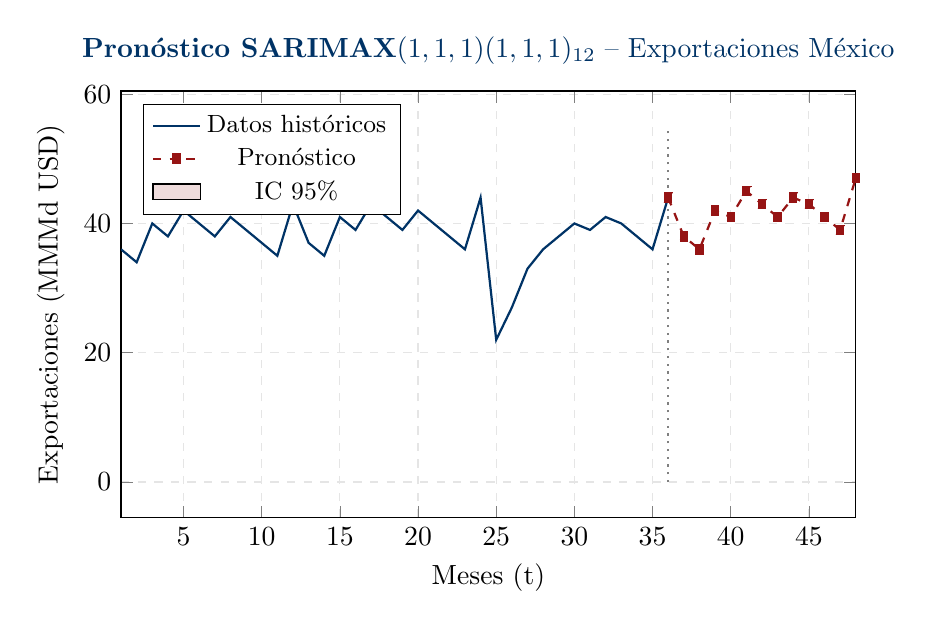
\begin{tikzpicture}
    \begin{axis}[
        width=0.9\textwidth, height=7cm,
        xlabel={Meses (t)},
        ylabel={Exportaciones (MMMd USD)},
        title={\textbf{Pronóstico SARIMAX$(1,1,1)(1,1,1)_{12}$} -- Exportaciones México},
        title style={color=upnavy},
        grid=major, grid style={dashed, gray!20},
        legend pos=north west,
        legend style={font=\small},
        xmin=1, xmax=48,
    ]
      % Datos históricos (simulados representativos)
      \addplot[thick, color=upnavy, mark=none] coordinates {
        (1,36)(2,34)(3,40)(4,38)(5,42)(6,40)(7,38)(8,41)(9,39)(10,37)(11,35)(12,43)
        (13,37)(14,35)(15,41)(16,39)(17,43)(18,41)(19,39)(20,42)(21,40)(22,38)(23,36)(24,44)
        (25,22)(26,27)(27,33)(28,36)(29,38)(30,40)(31,39)(32,41)(33,40)(34,38)(35,36)(36,44)
      };
      % Pronóstico puntual
      \addplot[thick, dashed, color=darkred, mark=square*, mark size=1.5] coordinates {
        (36,44)(37,38)(38,36)(39,42)(40,41)(41,45)(42,43)(43,41)(44,44)(45,43)(46,41)(47,39)(48,47)
      };
      % Banda de confianza superior
      \addplot[name path=upper, draw=none, color=darkred!30] coordinates {
        (36,44)(37,41)(38,40)(39,46)(40,45)(41,50)(42,48)(43,46)(44,49)(45,48)(46,47)(47,44)(48,53)
      };
      % Banda de confianza inferior
      \addplot[name path=lower, draw=none, color=darkred!30] coordinates {
        (36,44)(37,35)(38,32)(39,38)(40,37)(41,40)(42,38)(43,36)(44,39)(45,38)(46,35)(47,34)(48,41)
      };
      \addplot[fill=darkred!15] fill between[of=upper and lower];

      % Línea vertical que marca inicio del pronóstico
      \addplot[thick, dotted, color=gray] coordinates {(36,0)(36,55)};

      \legend{Datos históricos, Pronóstico, , , IC 95\%}
    \end{axis}
  \end{tikzpicture}
  \caption{Pronóstico a 12 meses del modelo SARIMAX$(1,1,1)(1,1,1)_{12}$.
    La línea vertical punteada separa la muestra de estimación del horizonte de pronóstico.
    La banda sombreada representa el intervalo de confianza al 95\%.}
  \label{fig:forecast}
\end{figure}

%===================================================================
\section{Metodología Box-Jenkins: Proceso Completo}
%===================================================================

La Figura~\ref{fig:boxjenkins} resume el proceso iterativo de Box-Jenkins para la
construcción de un modelo SARIMA/SARIMAX.

\begin{figure}[H]
  \centering
  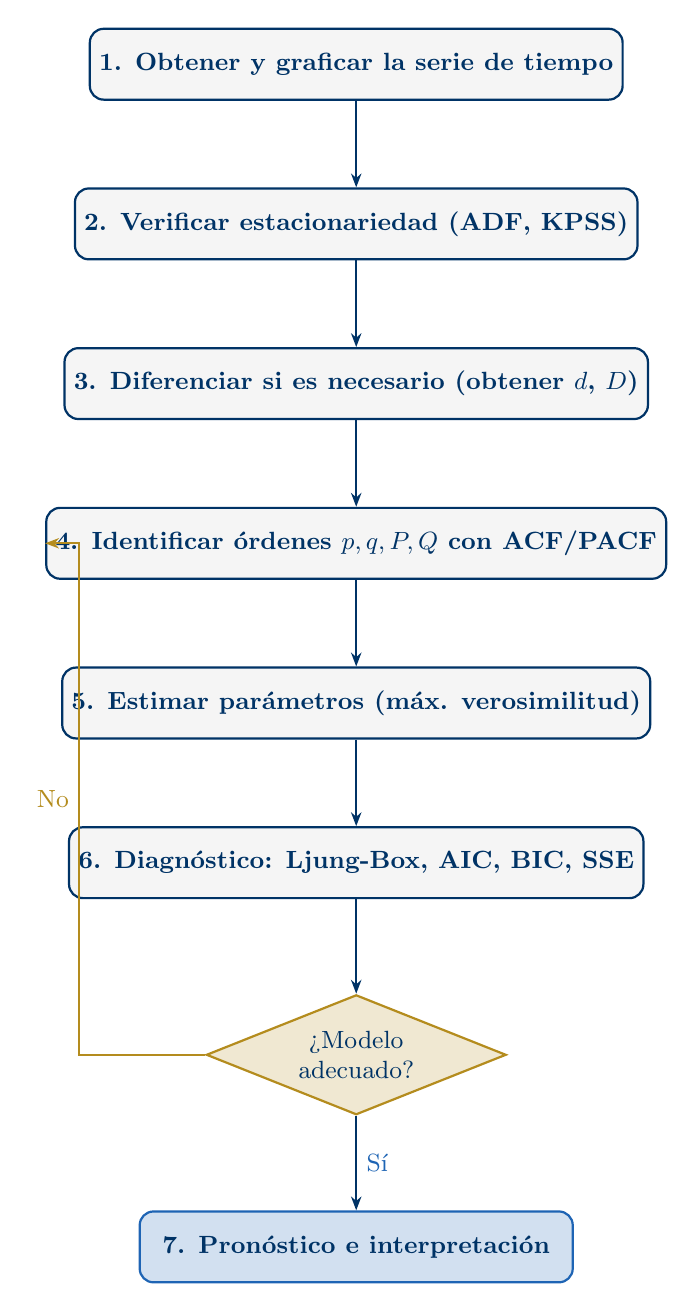
\begin{tikzpicture}[
      node distance=1.1cm,
      block/.style={draw=upnavy, fill=lightgray, rounded corners=5pt,
                    minimum width=5.5cm, minimum height=0.9cm,
                    align=center, font=\small\bfseries, text=upnavy, thick},
      decision/.style={draw=upgold, fill=upgold!20, diamond,
                       minimum width=3.5cm, minimum height=1.2cm,
                       align=center, font=\small, text=upnavy, thick,
                       aspect=2.5},
      arrow/.style={-{Stealth[length=5pt]}, thick, color=upnavy},
      yarrow/.style={-{Stealth[length=5pt]}, thick, color=upgold},
    ]
    \node[block] (data)    {1. Obtener y graficar la serie de tiempo};
    \node[block, below=of data]  (stat)  {2. Verificar estacionariedad (ADF, KPSS)};
    \node[block, below=of stat]  (diff)  {3. Diferenciar si es necesario (obtener $d$, $D$)};
    \node[block, below=of diff]  (ident) {4. Identificar órdenes $p,q,P,Q$ con ACF/PACF};
    \node[block, below=of ident] (estim) {5. Estimar parámetros (máx. verosimilitud)};
    \node[block, below=of estim] (diag)  {6. Diagnóstico: Ljung-Box, AIC, BIC, SSE};
    \node[decision, below=1.2cm of diag] (ok) {¿Modelo\\ adecuado?};
    \node[block, below=1.2cm of ok, fill=accentblue!20, draw=accentblue]
      (forecast) {7. Pronóstico e interpretación};

    \draw[arrow] (data)    -- (stat);
    \draw[arrow] (stat)    -- (diff);
    \draw[arrow] (diff)    -- (ident);
    \draw[arrow] (ident)   -- (estim);
    \draw[arrow] (estim)   -- (diag);
    \draw[arrow] (diag)    -- (ok);
    \draw[arrow] (ok)      -- node[right, font=\small, color=accentblue]{Sí} (forecast);

    % Flecha de retroalimentación
    \draw[yarrow] (ok.west) -- +(-1.6,0) |- node[left, font=\small, color=upgold,
      pos=0.25]{No} (ident.west);
  \end{tikzpicture}
  \caption{Metodología iterativa de Box-Jenkins para modelos SARIMA/SARIMAX}
  \label{fig:boxjenkins}
\end{figure}

%===================================================================
\section{Resumen y Conclusiones}
%===================================================================

\begin{table}[H]
  \centering
  \caption{Síntesis: Todo lo visto en clase sobre modelos SARIMA/SARIMAX}
  \label{tab:resumen}
  \rowcolors{2}{lightgray}{white}
  \begin{tabular}{>{\bfseries\color{upnavy}}p{3.5cm} p{10cm}}
    \toprule
    \rowcolor{upnavy}
    \textcolor{white}{Concepto} & \textcolor{white}{Descripción clave} \\
    \midrule
    Modelo SARIMA & $(S)$ARIMA$(p,d,q)(P,D,Q)_s$: combina componentes AR, I y MA
      en sus versiones regular y estacional \\
    Parámetro $q$ & Se identifica con la ACF; indica los rezagos MA \\
    Parámetro $p$ & Se identifica con la PACF (esperanza condicional); indica los rezagos AR \\
    Parámetro $d$ & Número de diferenciaciones regulares (stationarity via diff) \\
    Por qué no ACF para AR & La ACF aplicada a un proceso AR no corta abruptamente;
      por eso la PACF es la herramienta correcta \\
    Parsimonia & $p+d+q+P+D+Q \leq C$; se prefiere el modelo más simple \\
    AIC / BIC & Criterios de información que penalizan la complejidad; minimizar \\
    Log-verosimilitud & Mide el ajuste del modelo; maximizar \\
    SSE & Suma de cuadrados del error; minimizar \\
    Prueba Ljung-Box & Verifica que los residuales sean ruido blanco \\
    SARIMAX & Extensión con variables exógenas $\mathbf{X}_t$ \\
    \bottomrule
  \end{tabular}
\end{table}

Los modelos SARIMA y SARIMAX constituyen una herramienta poderosa para el análisis
de series de tiempo en finanzas cuantitativas. La correcta identificación de los
órdenes mediante ACF y PACF, combinada con el principio de parsimonia y los criterios
AIC/BIC/Ljung-Box, permite construir modelos robustos y con buen poder predictivo.

\vspace{1cm}
\hrule
\vspace{0.4cm}
{\small\textit{Documento elaborado para la materia de Series de Tiempo, Finanzas Cuantitativas,
Universidad Panamericana. Basado en las notas de clase de la Figura presentada.
Regina Flores Chávez --- Abril 2026.}}

\end{document}
